\section{BenchCouncil BigDataBench}
{{\footnotesize
\begin{description}[labelwidth=5em, labelsep=1em, leftmargin=*, align=left, itemsep=0.3em, parsep=0em]
  \item[date:] 2020-01-01
  \item[version:] TODO
  \item[last\_updated:] 2020-01
  \item[expired:] unknown
  \item[valid:] yes
  \item[valid\_date:] TODO
  \item[url:] \href{https://www.benchcouncil.org/BigDataBench/}{https://www.benchcouncil.org/BigDataBench/}
  \item[doi:] TODO
  \item[domain:] General
  \item[focus:] Big data and AI benchmarking across structured, semi-structured, and unstructured data workloads
  \item[keywords:]
    - big data
    - AI benchmarking
    - data analytics
  \item[summary:] BigDataBench provides benchmarks for evaluating big data and AI workloads with realistic datasets (13 sources) and pipelines across analytics, graph, warehouse, NoSQL, streaming, and AI.

  \item[licensing:] TODO
  \item[task\_types:]
    - Data preprocessing
    - Inference
    - End-to-end data pipelines
  \item[ai\_capability\_measured:]
    - Data processing and AI model inference performance at scale
  \item[metrics:]
    - Data throughput
    - Latency
    - Accuracy
  \item[models:]
    - CNN
    - LSTM
    - SVM
    - XGBoost
  \item[ml\_motif:]
    - General
  \item[type:] Benchmark
  \item[ml\_task:]
    - NA
  \item[solutions:] TODO
  \item[notes:] Built on eight data motifs; provides Hadoop, Spark, Flink, MPI implementations.

  \item[contact.name:] Jianfeng Zhan (BenchCouncil)
  \item[contact.email:] unknown
  \item[results.links.name:] ChatGPT LLM
  \item[results.links.url:] \href{https://docs.google.com/document/d/1VFRxhR2G5A83S8PqKBrP99LLVgcCGvX2WW4vTtwxmQ4/edit?usp=sharing}{https://docs.google.com/document/d/1VFRxhR2G5A83S8PqKBrP99LLVgcCGvX2WW4vTtwxmQ4/edit?usp=sharing}
  \item[fair.reproducible:] Yes
  \item[fair.benchmark\_ready:] Yes
  \item[ratings.software.rating:] 0
  \item[ratings.software.reason:] Not analyzed. 

  \item[ratings.specification.rating:] 9.0
  \item[ratings.specification.reason:] Evaluates AI at multiple levels (micro to end-to-end); tasks and workloads are clearly defined, though specific I/O formats and constraints vary.

  \item[ratings.dataset.rating:] 9.0
  \item[ratings.dataset.reason:] Realistic datasets across diverse domains; FAIR structure for many components, but individual datasets may not all be versioned or richly annotated.

  \item[ratings.metrics.rating:] 9.0
  \item[ratings.metrics.reason:] Latency, throughput, and accuracy clearly defined for end-to-end tasks; consistent across models and setups.

  \item[ratings.reference\_solution.rating:] 8.0
  \item[ratings.reference\_solution.reason:] Reference implementations for several tasks exist, but setup across all tasks is complex and not fully streamlined.

  \item[ratings.documentation.rating:] 8.0
  \item[ratings.documentation.reason:] Central documentation exists, with detailed component breakdowns; environment setup across platforms (e.g., hardware variations) can require manual adjustment.

  \item[id:] benchcouncil\_bigdatabench
  \item[Citations:] \cite{gao2018bigdatabenchscalableunifiedbig}
  \item[Ratings:]
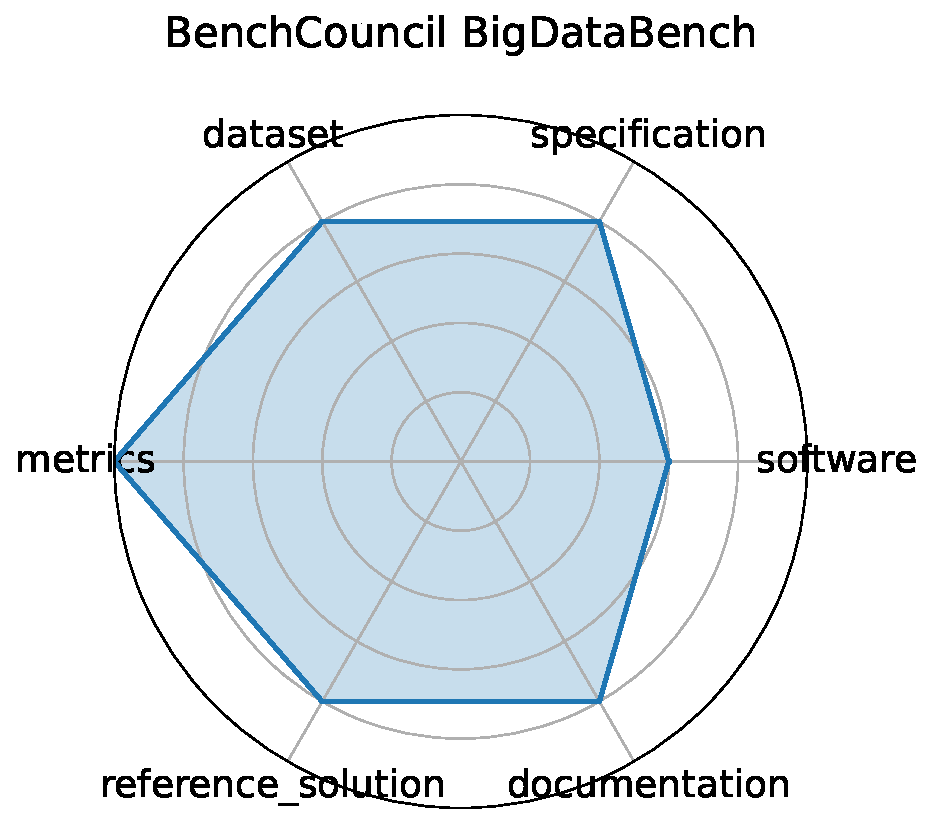
\includegraphics[width=0.2\textwidth]{benchcouncil_bigdatabench_radar.pdf}
\end{description}
}}
\clearpage